\section{Product perspective}
\subsection{Data State Diagram}
The collected data will certainly be the nucleus of the proposed system. The following state diagram displays the main actions that Data4Help will perform on the data, from the collection to an eventual access by a third party.\\ 
\begin{figure}[H]
    \renewcommand{\thefigure}{\alph{figure}}
    \makebox[\textwidth]{
        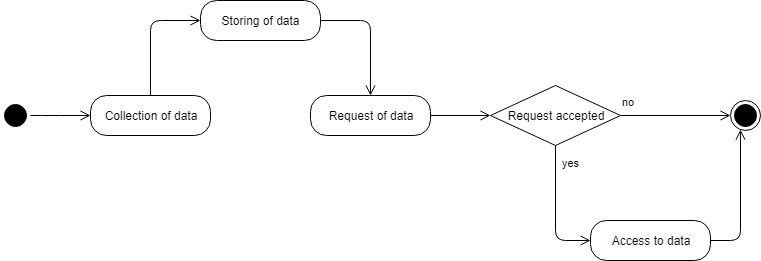
\includegraphics[width=1.4\linewidth]{images/State_Diagram.jpg}
    }
    \captionsetup{labelformat=parens, labelsep=space, name=}
    \caption{General data flow from the user to a requiring third party.}
\end{figure}

\subsection{UML Class Diagram}
The following class diagrams describe a possible model for the Data4Help and AutomatedSOS services:

\begin{landscape}
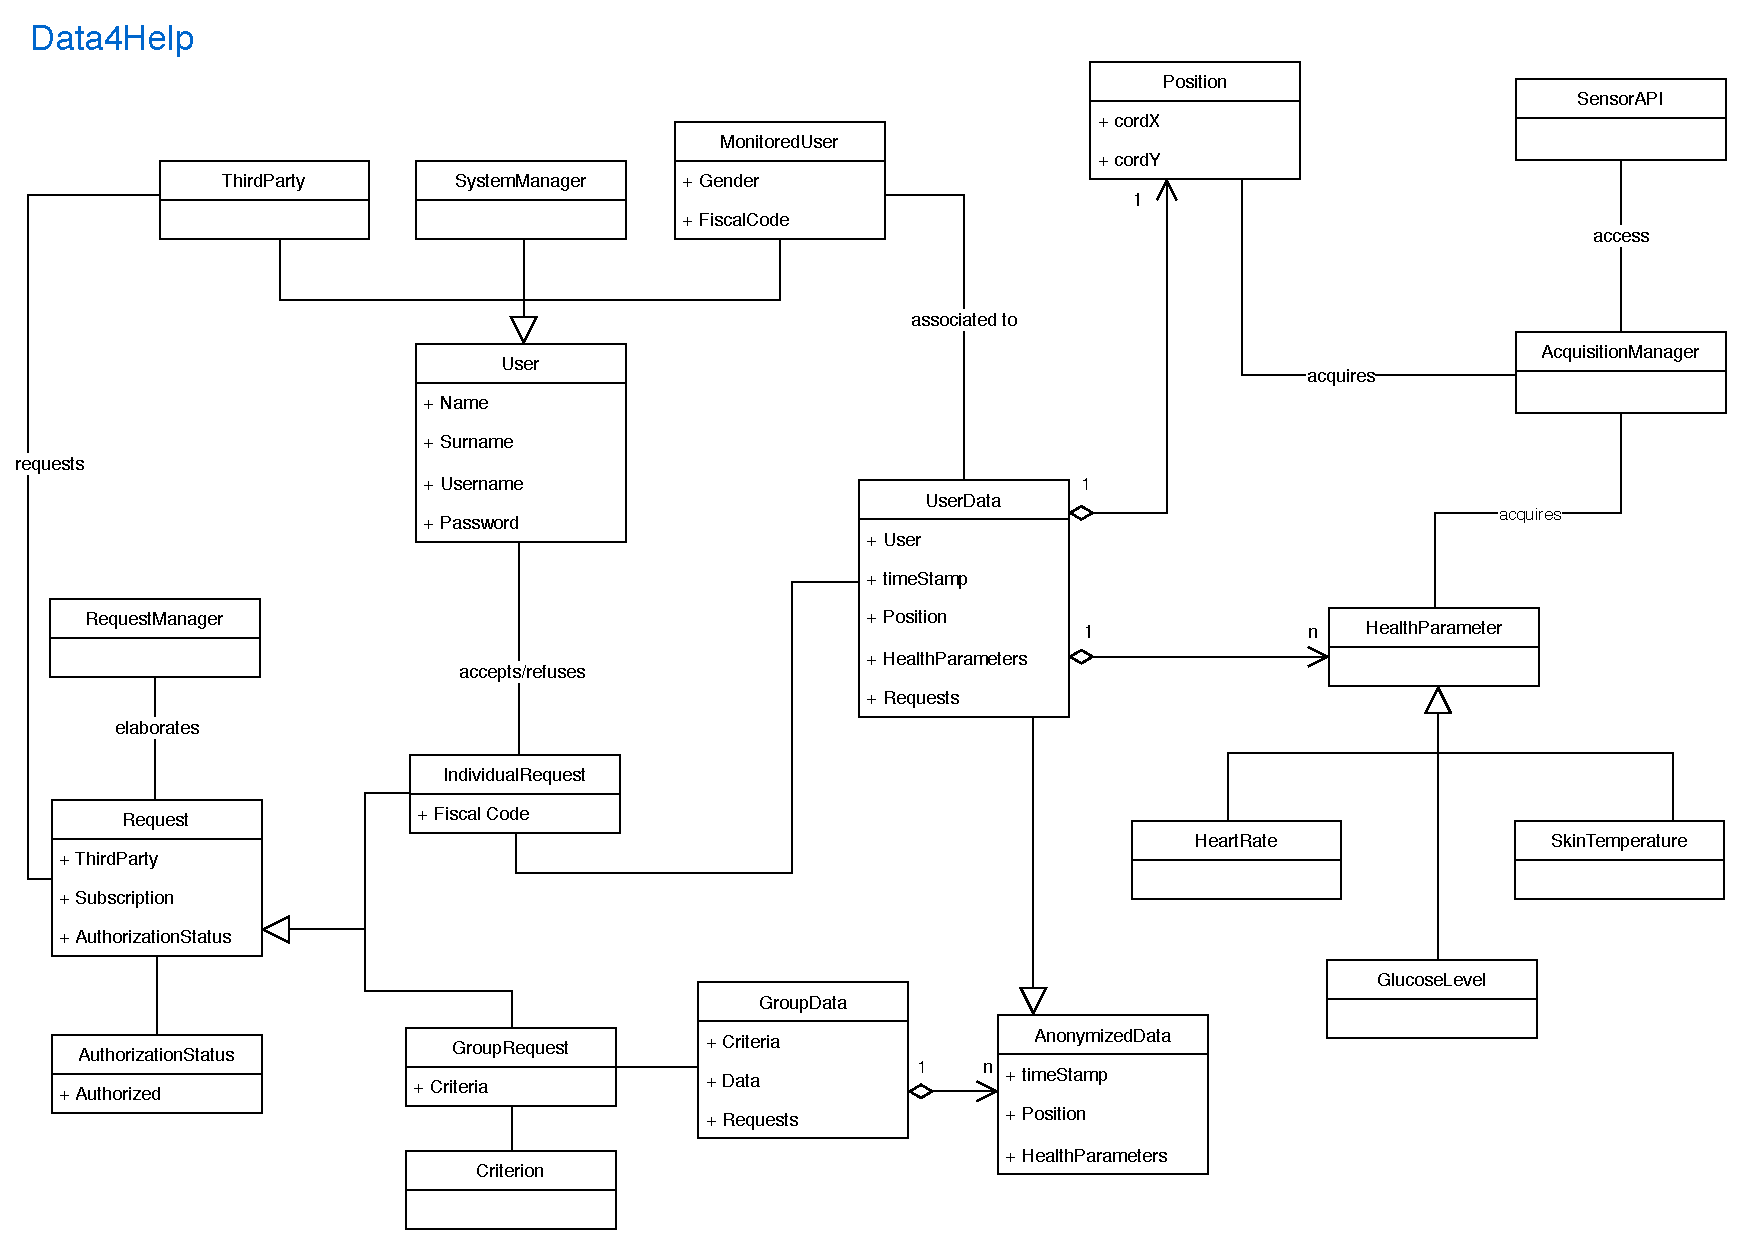
\includepdf[angle=90]{pdfs/UML_Data4Help.pdf}
\end{landscape}
\begin{landscape}
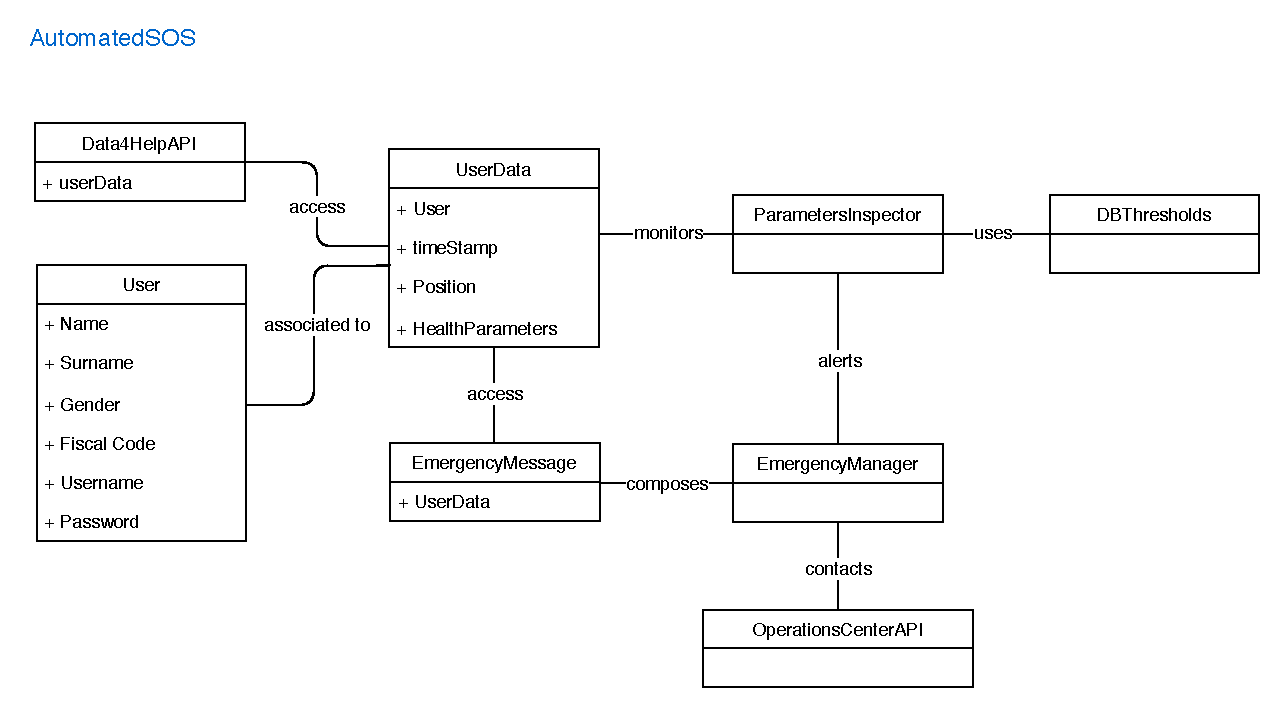
\includepdf[angle=90]{pdfs/UML_AutomatedSOS.pdf}
\end{landscape}

The diagrams showed above are intended as an high level representation of the essential features of the system. A detailed description of the communication infrastructure and the client applications will be given in the design and implementation phases.   

\section{Product functions}
    The following section lists the main functions offered by the system, focusing both on the end users and on the third parties.
    Of course, all the goals identified in the previous section will be offered as functions of the system-to-be.
    
    \subsection{Data4Help}
        \subsubsection {Data collection}
            The core function offered by Data4Help will be the real-time acquisition of the location and the health status of the users. The system will collect parameters such as GPS position, hearth rate and temperature through the sensors' interfaces in the device OS.
            All the data is permanently stored by the service and will be available to those who request them.
        
        \subsubsection {Third parties access to data}
            The system will let registered third parties to request an access to Data4Help data. This function can be divided in two categories: access to individual data and access to anonymized group of data. 
            Requests for individual data require to insert the SSN or Fiscal Code of the corresponding individual. \\
            The system will offer the possibility to customize a request for group data according to different criteria (age, gender, location, etc.).
            Third parties can also select the option of subscribing to the data, in order to receive them as soon as they are collected by Data4Help.
        
        \subsubsection {Accept or Refuse a request for data}
            When a third party requests the access to individual data, the system will notify the corresponding user and ask him/her to accept or decline the request. 
            The notification will show to the users the identity of the third party who requested their data.
        
    \subsection{AutomatedSOS}
        \subsubsection{Users health monitoring}
            Using Data4Help technology, AutomatedSOS will be able to monitor in real-time the heath status of its registered users. 
            The system will compare the parameters provided by Data4Help with predefined thresholds to detect the current condition of the users.
        
        \subsubsection {Emergency intervention}
            If the system detects an anomaly in the user's parameters, an emergency request will be sent to the Operations Center.
            AutomatedSOS will compose a message containing all the user's personal information, his/her current location and the health parameters list.  
            The ambulance intervention won't be managed by the system, that can only guarantee to contact the NHS within 5 seconds from the anomaly detection.  

\section{User characteristics}
    In general, users of our system are not expected to be particularly tech-savvy. It is assumed that the users are comfortable to interact with a basic application on a mobile device.
    On the other side, third parties are expected to have a broader technological back-ground, since they will interact with the data sent by the service.
    In particular, third parties who requests data of a group of people have to know how to manage the huge amount of data received by the system.
    
    \subsection{Actors}
    \begin{itemize}
        \item Visitor: a person that is not registered yet. The only action he/she can perform is enter the registration process.
        \item User: a person who has registered to the service and, after the login phase, can exploit all the functionalities provided by the system.
        \item System Manager: an employee of TrackMe in charge of maintaining and updating the system.
        Possible updates concerning Data4Help are changes in the privacy criteria for group requests and additions of new research categories.  Further updates are modifications of parameters' thresholds in AutomatedSOS.
        \item Third Party: an entity who is registered to the service with the purpose of accessing to data stored by the system.
        After the login phase it can request data of Data4Help users by filling the apposite form: it has to select some criteria for group requests and to insert a Fiscal Code if it wants to receive the data of a single user. 
        \item Operations Center employee: the NHS operator working at the Operations Center at the moment in which an emergency request arrives from AutomatedSOS. This actor establishes the emergency level and coordinates the ambulance intervention.  
    \end{itemize}
    
\section{Assumptions, dependencies and constraints}
\subsection{Domain Assumptions}
Data4Help:  
\begin{enumerate} [label={[D\arabic*]}]
    \item Users insert credentials that correspond to their identity.
    \item When a new registered user sends his/her credentials to the system, the message will be surely received.
    \item The communication channel doesn't corrupt the data sent by the user's device to the system and vice versa.
    \item The electronic device on which the system is installed is equipped with the GPS sensor.
    \item The electronic device on which the system is installed is equipped with the sensors related to the parameters tracked by Data4Help.
    \item The system retrieves the data from the sensors through the interfaces available on the electronic device.
    \item Position information provided by GPS is sufficiently accurate\cite{gps}.
    \item The sensors related to the health status collect the data with a reasonable precision.
    \item It's sufficient that the number of people involved in a group query is greater than 1000 people to ensure the users' privacy.
\end{enumerate}  
\noindent
AutomatedSOS:
\begin{enumerate} [resume, label={[D\arabic*]}]
    \item Data provided by Data4Help API are surely received and they are not corrupted.
    \item When an emergency request is sent to National Health Service, it surely receive it.
    \item When the National Health Service receives an emergency request, at least an ambulance is available.
    \item When parameters are below certain thresholds, it means that the user actually needs first aid.
    \item Operations Centers of the NHS are up 24/7.
    \item When the Operations Center gather a request from AutomatedSOS, it sends at least an ambulance and at least one arrives to the location of the emergency.
    \item NHS provides an API that allows third parties to send emergency requests in the form of an instant message received in their platform.
\end{enumerate}